\documentclass[10pt]{article}
\usepackage{graphicx}
\usepackage{tabularx}
\usepackage{verbatim}
\usepackage{listings}
\usepackage{longtable}

\title{ZAP Processor User Guide}
\author{Revanth Kamaraj} 

\begin{document}

\lstset{language=Perl}
\maketitle

\section{Introduction}

ZAP is a synthesizable open source 32-bit RISC processor core capable of 
executing ARM®v4T binaries at both the user and supervisor level. The processor 
features a 10-stage pipeline that allows it to reach reasonable operating 
frequencies. The processor supports standard I/D cache and memory management 
that may be controlled using coprocessor \#15. Both the cache and TLB are direct 
mapped. Caches, TLBs and branch memory are implemented as generic fully 
synchronous RAMs that can efficiently map to native FPGA block RAM to save FPGA 
resources. To simplify  device integration, the memory bus is fully compliant 
with Wishbone B3. A store buffer is implemented to improve performance.
\linebreak
\linebreak
NOTE: Please use pipeline retiming during synthesis for maximum timing performance. 

\subsection{CPU Clock and Reset}
ZAP uses a single clock called the core clock to drive the entire design. The 
clock must be supplied to the port I\_CLK. ZAP expects a rising edge 
synchronous I\_RESET (active high) to be applied i.e., 
the reset signal must change only on the rising edges of clock. The reset 
must be externally synchronized to the core clock before being applied to 
the processor.

\subsection{Block Digram}
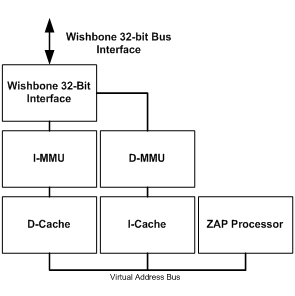
\includegraphics{images/image004.png}

\subsection{Pipeline Overview}

\begin{tabularx} {\linewidth}{|r|X|}
\hline

Stage & 
Description \\ \hline 

Fetch & 
Clocks data from I-cache into instruction register. Also branch predictor memory 
is read out in this stage. \\ \hline 

FIFO &
Instructions and corresponding PC+8 values are clocked into a shallow buffer.
 \\ \hline

Thumb Decoder &
Converts 16-bit instructions to 32-bit ARM instructions. Instructions predicted 
as taken cause the pipeline to change to the new predicted target. \\ \hline

Predecode &
Handles coprocessor instructions, SWAP and LDM/STM. \\ \hline

Decode &
Decodes ARM instructions. \\ \hline

Issue &
Operand values are extracted here from the bypass network. In case data from 
the bypass network is not available, the register file is read. \\ \hline

Shift &
Performs shifts and multiplies. Contains a single level bypass network to 
optimize away certain dependencies. Multiplication takes multiple clock cycles. \\ \hline

Execute &
Contains the ALU. The ALU is single cycle and handles arithmetic and logical 
operations. \\ \hline

Memory &
Clocks data from the data cache into the pipeline. Aligns read data as 
necessary. \\ \hline

Writeback &
Writes to register file. Can sustain 2 writes per clock cycle although the 
only use for the feature is accelerate LDR performance in the current 
implementation. \\ \hline
\end{tabularx}
\\
\\
ZAP features a 10 stage pipeline. The pipeline has an extensive bypass network 
to minimize pipeline stalls. A load accelerator allows data to be forwarded 
from memory a cycle early. Most non-multiply instructions can be executed 
within a single clock tick with no stalls. Exceptions to this rule are when 
multiplies or non-trivial shifts are used.
\\
\\
The following code takes 3 cycles to execute because R1 needs to be shifted 
and is not available until the first instruction enters the ALU: 
\\
\\
ADD R1, R2, R3 \\
ADD R4, R5, R1 LSL R2 \\
\\
\\
If the second register is not source shifted by a register that depends on the 
previous instruction, a data dependency check may be relaxed (Register R9 for 
the second instruction can be obtained in issue itself so nothing is blocking 
the second instruction from using the shifter) and thus the following code 
takes 2 cycles to execute:
\\
\\
ADD R1, R2, R3 LSL R5 \\
ADD R4, R1, R9 LSL R2 \\
\\
\\
Another feature of the pipeline is that it can issue memory operations with 
writeback in a single cycle. The following instructions takes 2 cycles to 
execute assuming a perfect cache.
\\ 
\\
LDR R0, [R1, \#2]! \\
ADD R1, R3, R4 LSL R1 \\
\\
\\
The pipeline feedback unit is designed to reasonably minimize pipeline stalls. 
Note however that pipeline bubble squashing is available only  across the 
instruction FIFO.

\subsection{Features}

\begin{itemize}
\item Fully synthesizable Verilog-2001 core.   
\item          Store buffer for improved performance.   
\item          Can execute ARMv4T code at both the user and supervisor level. 
\item          Wishbone B3 compatible interface. Cache unit supports burst access.
\item          10-stage pipeline design. Pipeline has bypass network to resolve 
               dependencies.
\item          2 write ports for the register file to allow LDR/STR with 
               writeback to execute as a single instruction. Note that the 
               register file is implemented using flip-flops.
\item          Branch prediction supported. Uses a 2-bit state for each branch.
\item          Split I and D writeback cache (Size can be configured using parameters).
\item          Split I and D MMUs (TLB size can be configured using parameters).
\item          Base restored abort model to simplify data abort handling.
\end{itemize}

\subsection{Branch prediction mechanism}

ZAP uses a relatively simple branch prediction mechanism (Note that the branch 
table block RAM is read in Fetch). Note that when using ARM code, the amount of 
branch table entries is cut by half since the lower 2 bits of PC are 0. A 
simple state machine is used to reinforce or modify the status of a branch. The 
pass and fail signals are generated from the ALU.

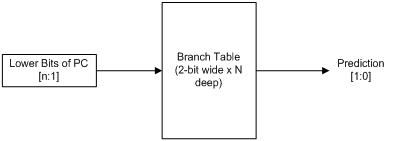
\includegraphics{images/image008.png}
\\
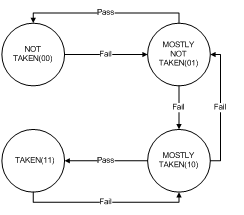
\includegraphics{images/image010.png}

\subsection{Cache/TLB Overview}

ZAP uses direct mapped cache (separate I/D) that is virtual. For decent 
performance, the cache is writeback. To enable writeback, each cache line has 
a dirty bit. The size of each cache line is fixed at 16 bytes. Since ARMv4 
specifies three kinds of paging schemes: section, large and small pages, 3 
TLB block RAMs are employed which are also direct mapped. ZAP has independent 
instruction and data caches/TLBs. The cache/MMU setup is v4 compatible. The 
cache should be enabled as soon as possible for good performance because the 
memory subsystem is efficient for burst transactions.

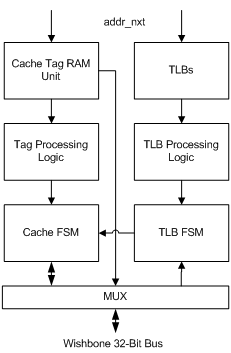
\includegraphics{images/image012.png}

\subsection{Running Simulations}
\subsubsection{Creating and Simulating Test Cases}

To create a test case, create a some assembly(.s extension) and 
C files(.c extension) and a linker script(.ld extension) in the directory 
\texttt{src/ts/$\langle$TestCase$\rangle$/}
\\
\\
Copy the \texttt{makefile} and \texttt{Config.cfg} from one of the existing test case directories 
to the directory texttt{src/ts/$\langle$TestCase$\rangle$/}. Edit the \texttt{Config.cfg} to suit the testcase.
\\
\\
To run simulations using the scripts provided, you will need Icarus 
Verilog 10.0 or higher and 32-bit libraries installed. Object files and 
waveform dumps can be found in the \texttt{obj/ts/$\langle$TestCase$\rangle$/} directory.
\\
\\
Enter \texttt{src/ts/$\langle$TestCase$\rangle$} and type \texttt{make}.
\\
\\
To clean object files, enter \texttt{src/ts/$\langle$TestCase$\rangle$} and type \texttt{make clean}.
\\
\\
NOTE: You can set the testbench and processor configuration in the \texttt{Config.cfg} 
file that contains a Perl hash. This file is present in the same directory as 
the test case. 
\\
\\
Here's a sample of what the \texttt{Config.cfg} file should contain.
\\
\\
\begin{lstlisting}[frame=none] % Perl code block start.

%Config = ( 
# CPU configuration.
DATA_CACHE_SIZE          => 4096,# Data cache size in bytes
CODE_CACHE_SIZE          => 4096,# Instruction cache size in bytes
CODE_SECTION_TLB_ENTRIES => 8,   # Instruction section TLB entries.
CODE_SPAGE_TLB_ENTRIES   => 32,  # Instruction small page TLB entries.
CODE_LPAGE_TLB_ENTRIES   => 16,  # Instruction large page TLB entries.
DATA_SECTION_TLB_ENTRIES => 8,   # Data section TLB entries.
DATA_SPAGE_TLB_ENTRIES   => 32,  # Data small page TLB entries.
DATA_LPAGE_TLB_ENTRIES   => 16,  # Data large page TLB entries.
BP_DEPTH                 => 1024,# Branch predictor depth.
INSTR_FIFO_DEPTH         => 4,   # Instruction buffer depth.
STORE_BUFFER_DEPTH       => 8,   # Store buffer depth.
SYNTHESIS                => 1,   # Make this to 1 to simulate compile 
                                 # from a synthesis perspective.

# Testbench configuration.
EXT_RAM_SIZE      => 32768, # External RAM size in bytes.
SEED              => -1,    # Seed. Use -1 to use random seed.
DUMP_START        => 2000,  # Starting memory address from which to dump.
DUMP_SIZE         => 200,   # Length of dump in bytes.
MAX_CLOCK_CYCLES  => 100000,# Clock cycles to run the simulation for.
ALLOW_STALLS      => 1,     # Make this 1 to allow 
                            # external RAM to signal a stall.
DEFINE_TLB_DEBUG  => 0,     # Make this 1 to define 
                            #TLB_DEBUG. Useful for debugging the TLB.

# Make this an anonymous has with entries like 
# "r10" => "32'h0" etc. These represent register 
# values at the end of simulation.
REG_CHECK                   => {"r1" => "32'h4", 
                                "r2" => "32'd3"},      

# Make this an anonymous hash with entries like 
# verilog_address => verilog_value etc.
FINAL_CHECK                 => {"32'h100" => "32'd4", 
                                "32'h66" => "32'h4"}       
);

\end{lstlisting}

\section{IO Ports and Configuration}

\begin{tabularx} {\linewidth}{|r|r|X|}
\hline
Signal Name & IO & Description \\ \hline

I\_CLK &
I &
Core clock. \\ \hline

I\_RESET &
I &
Core reset. \\ \hline

O\_WB\_CYC &
O &
Wishbone CYC signal. \\ \hline

O\_WB\_STB &
O & 
Wishbone STB signal. \\ \hline

O\_WB\_ADR[31:0] &
O &
Wishbone 32-bit address. \\ \hline

O\_WB\_SEL[3:0] &
O &
Wishbone byte lane enables. \\ \hline

O\_WB\_WE &
O &
Wishbone write enable. \\ \hline

O\_WB\_DAT[31:0] &
O &
Wishbone write data. \\ \hline

O\_WB\_CTI[2:0] &
O &
Wishbone cycle type indicator. \newline
0b010 = Incrementing burst. \newline
0b111 = End of burst. \newline
The interface shall only generate one of the above 2 codes. 
A single transfer is effectively a burst of length 1.\\ \hline

O\_WB\_BTE[1:0] &
O &
Burst type extension tag. This always reads 0x0 to indicate that
the processor can only perform incrementing linear bursts (32-bit width). 
\\ \hline

I\_WB\_DAT[31:0] &
I &
Wishbone read data. \\ \hline

I\_WB\_ACK &
I &
Wishbone acknowledge. \\ \hline

I\_IRQ &
I  &
IRQ Interrupt. \\ \hline

I\_FIQ &
I &
FIQ Interrupt. \\ \hline
\end{tabularx}
\\
\\
Verilog parameters can be used to statically configure the processor instance
as shown in the table below.
\\
\\
\begin{tabularx}{\linewidth}{|r|X|X|}
\hline
Parameter &
Description &
Notes \\ \hline

DATA\_CACHE\_SIZE[31:0] &
Data cache size in bytes. &
1 \\ \hline

CODE\_CACHE\_SIZE[31:0] &
Instruction cache size in bytes. &
1 \\ \hline

CODE\_SECTION\_TLB\_ENTRIES[31:0] &
Section TLB entries (CODE). &
2 \\ \hline

CODE\_SPAGE\_TLB\_ENTRIES[31:0] &
Small page TLB entries (CODE). &
2 \\ \hline

CODE\_LPAGE\_TLB\_ENTRIES[31:0] &
Large page TLB entries (CODE). &
2 \\ \hline

DATA\_SECTION\_TLB\_ENTRIES[31:0] &
Section TLB entries (DATA). &
2 \\ \hline

DATA\_SPAGE\_TLB\_ENTRIES[31:0] &
Small page TLB entries (DATA). &
2 \\ \hline

DATA\_LPAGE\_TLB\_ENTRIES[31:0] &
Large page TLB entries (DATA). &
2 \\ \hline

FIFO\_DEPTH[31:0] &
Depth of the fetch buffer in the pipeline. &
3 \\ \hline

BP\_ENTRIES[31:0] &
Depth of the branch predictor memory. &
3 \\ \hline

STORE\_BUFFER\_DEPTH[31:0] &
Set the depth of the store buffer. Do not set it to a value less than 16. &
4  \\ \hline
\end{tabularx}

NOTE. \\

1. Should be a power of 2 and greater than 128 bytes. \\

2. Should be a power of 2 and must be at least 2 entries. \\
 
3. Should be a power of 2 and must be greater than 2. \\

4. Depth must be 16 or more and a power of 2. \\
\\

\section{CP15 commands}

ZAP features an ARMv4 compatible cache subsystem (cache and MMU). This subsystem 
may be configured by issuing commands to specific CP \#15 registers using 
coprocessor instructions. A list of supported CP \#15 commands/registers are 
listed in the table below:
\\
\\
WARNING: In particular, cleaning and flushing of specific locations is not 
supported. The OS should avoid issuing such commands.
\\
\\
\begin{longtable}{|p{0.5cm}|p{2cm}|p{6cm}|p{0.5cm}|}
\hline

Reg. & Name & Description & Note \\ \hline

0 &
ID &
[23:16] – Always reads 0x01 to indicate a v4 implementation. \newline
Other bits are UNDEFINED. &
1 \\ \hline

1 &
CON &
[0] – MMU enable. \newline
[2] – Data cache enable. \newline
[8] – S bit. \newline
[9] – R bit. \newline
[12] – Instruction cache enable. \newline
READ ONLY bits are described in note 2. \newline
Bits other than the ones specified here and in note 2 are UNDEFINED. \newline
2 \\ \hline

2 &
TRBASE &
Holds 16KB aligned base address of L1 table. &
 \\ \hline

3 &
DAC &
Domain Access Control Register. &
 \\ \hline
 
5 &
FSR &
Fault address register. &
4 \\ \hline

6 &
FAR &
Fault status register. &
4 \\ \hline

7 &
CACHECON &
Data written to this register should be zero else UNDEFINED operations can occur. \newline
\begin{tiny}
CACHECON control table. \newline
        {\begin{tabularx}{\linewidth}{|X|X|X|} 
         \hline
         Opcode2 &
         CRm &
         Description \\ \hline
         \hline
         000 &
         0111 &
         Flush all caches. \\ \hline
         
         000 &
         0101 &
         Flush I cache. \\ \hline
         
         000 &
         0110 &
         Flush D cache. \\ \hline
         
         000 &
         1011 &
         Clean all caches. \\ \hline
         
         000 &
         1010 &
         Clean D cache. \\ \hline
         
         000 &
         1111 &
         Clean and flush all caches. \\ \hline
         
         000 &
         1110 &
         Clean and flush D cache. \\ \hline
         \end{tabularx}} \end{tiny} &

3 \\ \hline

8 &
TLBCON &
Data written to this register should be zero else UNDEFINED operations can occur. \newline
TLBCON Control table.\newline
        {\begin{tabularx}{\linewidth}{|X|X|X|}
        \hline
        Opcode2 &
        CRm &
        Description \\ \hline
        \hline
        
        000 &
        0111 &
        Flush all TLBs \\ \hline
        
        000 &
        0101 &
        Flush I TLB. \\ \hline
        
        000 &
        0110 &
        Flush D TLB. \\ \hline
        \end{tabularx}} &
 
3 \\ \hline
\end{longtable}

NOTE:

1. Read only. Writes have NO effect. \newline

2. Processor does not check for address alignment ([1] reads 0), only supports 
Little Endian access, full 32-bit, write buffer always enabled ([7:4] reads 0b0011), 
does not support high vectors ([13] reads 0) and always has a predictable cache 
strategy ([11] reads 1) i.e., direct mapped. \newline

3. Reads are UNPREDICTABLE. \newline

4. Only data MMU can update this. For debug purposes, these are RW registers. \newline

\end{document}

